\documentclass[pdf]{beamer}
\usepackage{times}
\usepackage{polski}
\usepackage[utf8]{inputenc}
\usepackage[T1]{fontenc}
\usetheme{Pittsburgh}
\usecolortheme{wolverine}
\usefonttheme{serif}
\mode<presentation>{}
\title{Rola platformy Instagram w odbiorze własnego wyglądu:}
\subtitle{Badanie zależności między modyfikowaniem swojego wizerunku, a oceną postrzegania swojego ciała wśród kobiet}
\author{Sara Pasturczak, Aleksandra Popowska, Wiktor Warchałowski\\Gdański Uniwersytet Medyczny}
\date{24 Maja 2022}

\begin{document}

\begin{frame}
  \titlepage
\end{frame}

\begin{frame}{Wprowadzenie}
\begin{center}
Dotychczasowe badania przedstawiały różne, sprzeczne ze sobą wyniki, iż platformy społecznościowe zwiększają, zmniejszają lub w ogóle nie wpływają na samoakceptację. Z tego powodu, celem niniejszego artykułu jest sprawdzenie czy modyfikowanie zdjęć własnego wizerunku na platformie Instagram ma związek z poziomem zadowolenia z własnego ciała u młodych kobiet
\end{center}
\end{frame}

\begin{frame}{Materiały i metoda}
\begin{center}
Badanie zostało przeprowadzone przy użyciu Kwestionariuszy Google. Wykorzystany został 10-itemowy kwestionariusz Body Appreciation Scale 2 (BAS-2) T. Tylka i N. Wood-Barcalow w polskiej adaptacji M. Razmus i W. Razmus. \\
Dane uzyskane w kwestionariuszu zostały zsumowane i na tej podstawie zostały porównane dwie grupy badanych (osoby modyfikujące oraz niemodyfikujące swoich zdjęć umieszczanych na platfromie Instagram).
\end{center}
\end{frame}

\begin{frame}{Wyniki}
\begin{table}[h!]
\caption{\textit{Wyniki podstawowych parametrów statystyki opisowej}}
\begin{tabular}{lccccccc}
\textbf{Modyfikacja} & \textbf{N}                                        & \textbf{Średnia}                                    & \textbf{Mediana}                                    & \textbf{\begin{tabular}[c]{@{}c@{}}Odchylenie\\ Standardowe\end{tabular}} & \textbf{Max}                                      & \textbf{Min}                                      & \textbf{Rozstęp}                                  \\
Tak                  & {\color[HTML]{333333} 25}                         & {\color[HTML]{333333} 32.7}                         & {\color[HTML]{333333} 32}                          & {\color[HTML]{333333} 9.6}                                                 & {\color[HTML]{333333} 49}                         & {\color[HTML]{333333} 11}                         & {\color[HTML]{333333} 38}                         \\
Nie                  & \cellcolor[HTML]{F2F2F2}{\color[HTML]{333333} 51} & \cellcolor[HTML]{F2F2F2}{\color[HTML]{333333} 32.7} & \cellcolor[HTML]{F2F2F2}{\color[HTML]{333333} 34} & \cellcolor[HTML]{F2F2F2}{\color[HTML]{333333} 9.59}                         & \cellcolor[HTML]{F2F2F2}{\color[HTML]{333333} 50} & \cellcolor[HTML]{F2F2F2}{\color[HTML]{333333} 11} & \cellcolor[HTML]{F2F2F2}{\color[HTML]{333333} 39}
\end{tabular}
\end{table}
\\
\begin{figure}[h!]
\centering
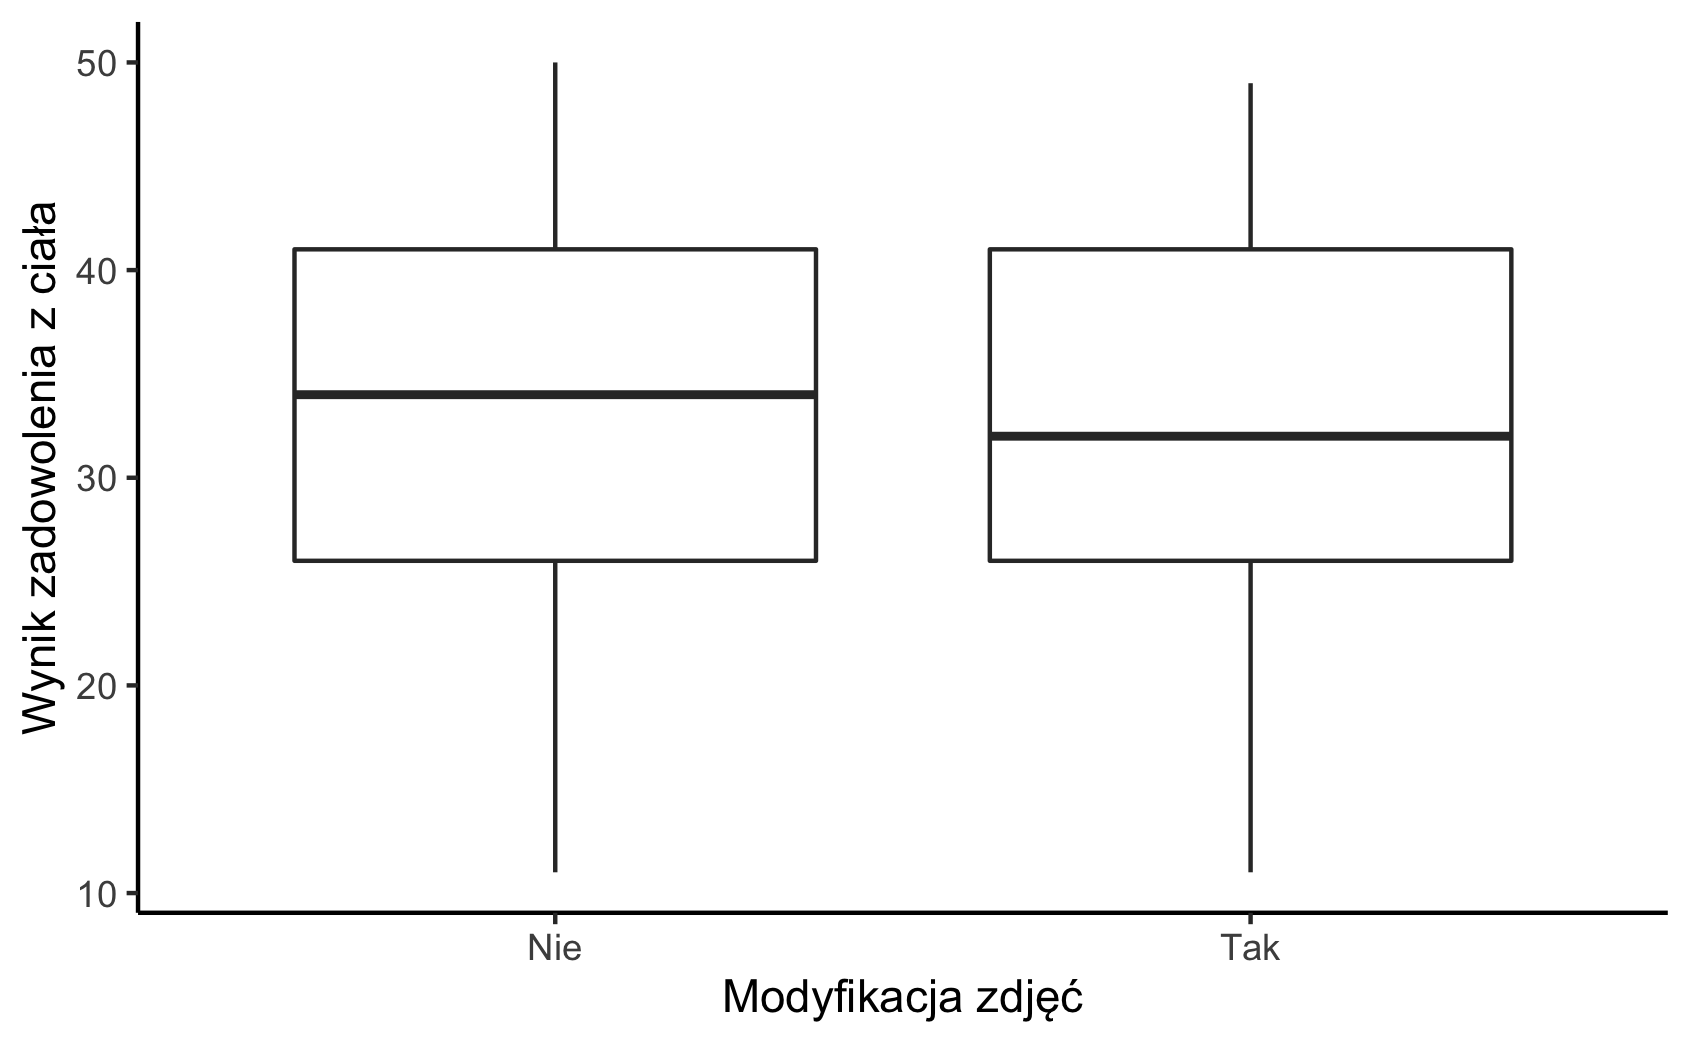
\includegraphics[scale=0.05]{boxwhisk}
\end{figure}
\end{frame}

\begin{frame}

\end{frame}

\end{document}